\subsection{Complex Impedance and AC Circuits} 

Answers to M\Alph{subsection} problems are on page \pageref{Z_and_AC_prob_answers}.  \textbf{\textcolor{red}{Updated \DTMnow.}}

%--------------------------------------------------------------------------------------------------------------
\begin{Exercise}
In the circuit to the right, the switch is closed at time $t=0.$  
(a)~Find the current $I_L$ through the 
	\begin{wrapfigure}[5]{r}{0.25\textwidth}
\vspace{-0.2in}\hfill	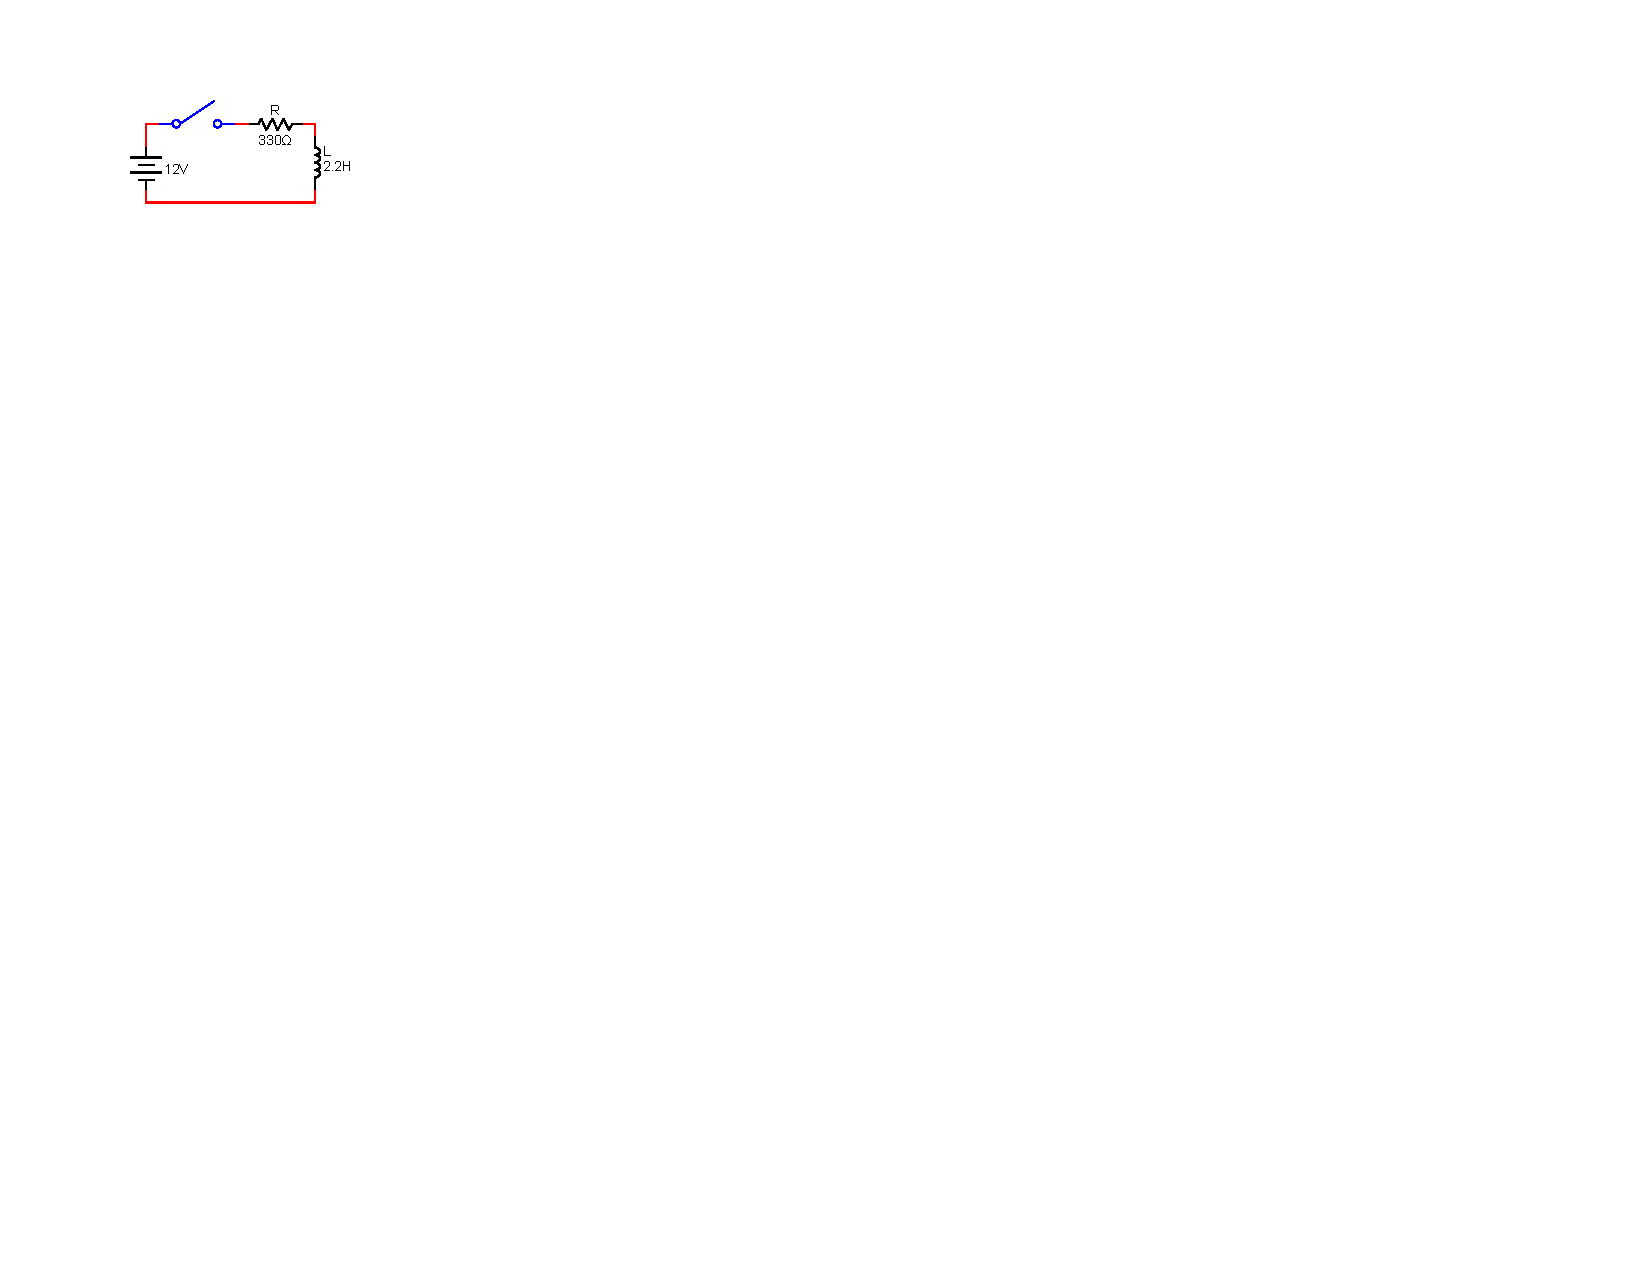
\includegraphics{M_problems/Z_and_AC/RL_circuit.pdf}
	\end{wrapfigure}
inductor at $t=10$~msec.  
(b)~Is the current through the resistor $I_R$ the same as through the inductor at that time?  
(c)~Find the voltage across the inductor $V_L$ at that time.  \textit{Hint: you should have found in Lab~\textsl{\ref{lab_inductors}} that the time constant for an ``LR'' circuit is given by $\tau=L/R$.}
\end{Exercise}
\begin{Answer}
(a) 28.2 mA (b) Yes, they are always the same.  If they weren't, then components would build up static charges and start attracting each other with large Coulomb forces, which among other things would be extremely dangerous! (c)~2.68~V
\end{Answer}


%--------------------------------------------------------------------------------------------------------------
\begin{Exercise}
This problem is an exact analog to the example we did in class, and which I have posted as an example problem on Blackboard.  Consider the circuit to the right, with a sinusoidal voltage source $V_S (t)=V_0 e^{i\omega t}.$  
	\begin{wrapfigure}[7]{r}{0.20\textwidth}
\vspace{-0.1in}\hfill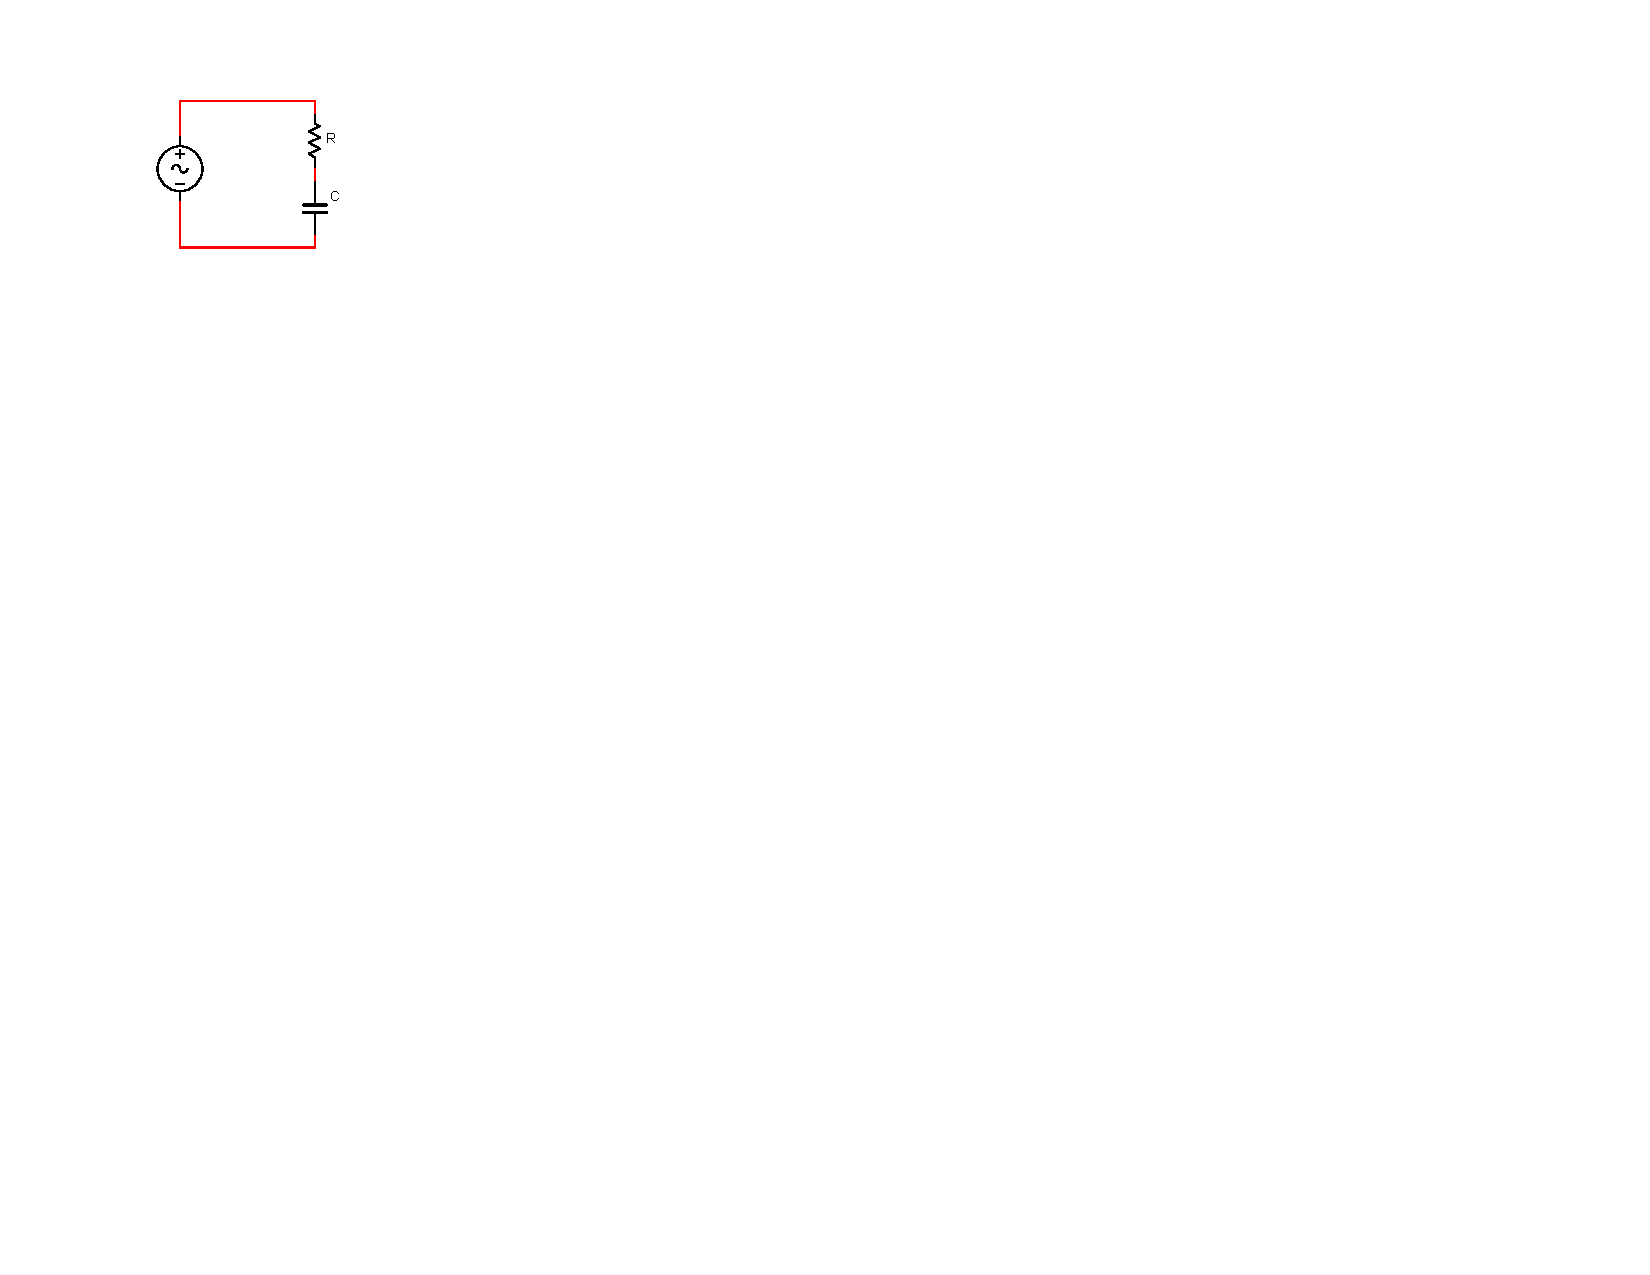
\includegraphics{M_problems/Z_and_AC/RC_circuit.pdf}
	\end{wrapfigure}
(a)~Find the magnitude and phase of the current $I(t)$ in the circuit.  (Both depend on $\omega$.)
(b)~Are the current $I_R$ through the resistor and the current $I_C$ through the capacitor in phase with each other?
(b)~Find the magnitude and phase of the voltage $V_C$ across the capacitor.  
(c) Find the ``cutoff frequency'' $f_c$ at which the ratio of  $\left| V_C \right| / V_0 =1 / \sqrt{2}$, or about 0.707.  
(d)~At this frequency, what is $ \left| V_C \right| / V_0$ expressed in decibels?  
(e)~Find expressions for $ \left| V_C \right| / V_0$ in the limit of low frequency and in the limit of high frequency to leading order.%
\footnote{Finding a limit \textit{to leading order} means that your answer should include one nonzero term.  
For instance, far away from two point charges $q_1$ and $q_2$, the electric field \textit{to leading order} is 
${\displaystyle  \lim_{r \to \infty} E(r)=\frac{k_e \left( q_1+q_2 \right) }{r^2} }.$
While $\displaystyle\lim_{r \to \infty} E(r)=0$ is true, the limit \textit{to leading order} provides the additional information that $E\sim 1/r^2$ at large distances.
}
(f)~Draw vectors on the complex plane for $V_S, V_R, V_C,$ and $I$ at time $t=0$.
\end{Exercise}
\begin{Answer}
(a) $|I|=V_0/\sqrt{R^2+1/(\omega C)^2 };~\phi=\tan^{-1}(1/\omega RC)$  
(b)~Yes, currents of components in series are \textit{always} in phase.
(c)~$|V_C |=V_0/\sqrt{(\omega RC)^2+1};~\phi=-\tan^{-1}(\omega RC) $
(d)~$f_c=\frac{\pi}{2}RC$ (e)~about $-3$~dB 
(f) As $\omega \to 0, V_C/V_0 \to 1$. As $\omega \to \infty, V_C/V_0 \sim (\omega RC)^{-1}.$  
\end{Answer}



%Ideas for additional problems:
%\vfill
%\pagebreak[3]

\vspace{0.7in}

\textbf{Answers to Selected {\thesubsection} Problems:}
\label{Z_and_AC_prob_answers}
%\shipoutExercise
\shipoutAnswer

\cleardoublepage
